L'utilisateur, afin de lancer une simulation, passera par une interface graphique. Voici un prototype possible pour l'interface voulue :



\vspace{5 mm}
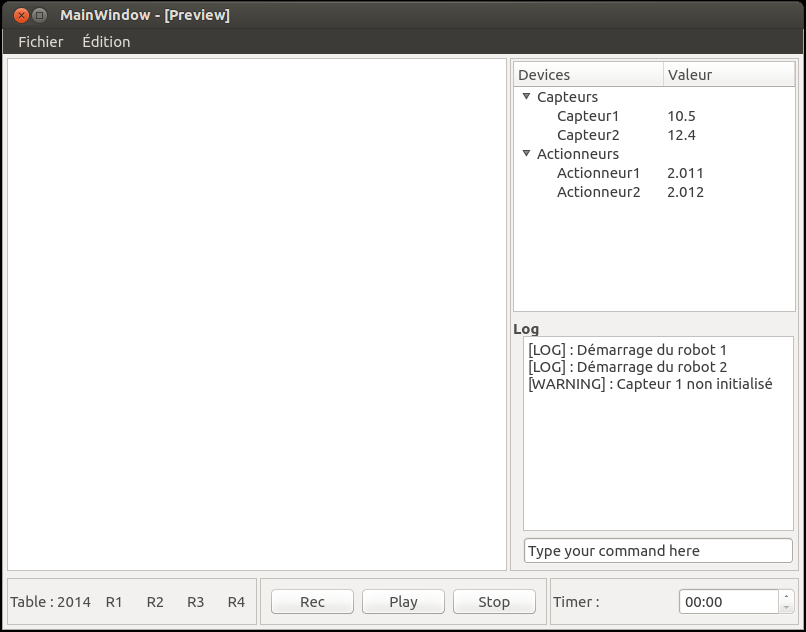
\includegraphics[scale=0.5]{GUI.png}
\vspace{5 mm}
\\

Cette interface devra proposer les fonctionnalités suivantes : 

\subsection{Besoins fonctionnels}

\subsubsection{Arborescence des onglets fichier et édition}
\textbf{Fichier}
\begin{itemize}
\item Nouveau
\item Ouvrir
\item Enregistrer sous
\item Enregistrer
\end{itemize}

\textbf{\'Edition}
\begin{itemize}
\item Insertion
    \begin{itemize}
    \item Objet
    \item Erreur $\rightarrow$ Choix du capteur ou de l'actionneur et de la nouvelle Valeur
%%    \item 
%%    \item 
    \end{itemize}

\item Table
\begin{itemize}
\item {Choix du Fichier de Description $\rightarrow$ Choix de l'Année} \footnote{"$\rightarrow$" signifie qu'une fenêtre s'ouvre pour réaliser l'action}
\end{itemize}
\item Supprimer Table

\item Ajouter un robot
    \begin{itemize}
    \item Robot 1 $\rightarrow$ Choix du fichier de description
    \item Robot 2 $\rightarrow$ Choix du fichier de description
    \item Robot 3 $\rightarrow$ Choix du fichier de description
    \item Robot 4 $\rightarrow$ Choix du fichier de description
    \end{itemize}
\item Supprimer Robot ( une fenêtre s'ouvre pour le choix des robots à supprimer )
%\item 
\end{itemize}

% \textbf{Affichage}
% \begin{itemize}
% \item Insertion
%     \end{itemize}
% \begin{itemize}
% \item Ajouter un robot
    
%\end{itemize}

\subsubsection{Afficher l'environnement en 2D vu du dessus}
%N ET T
Afin de suivre facilement l'avancement de la simulation, l'utilisateur doit avoir un retour visuel simple de la simulation. Le but de cet affichage est de proposer une vue pertinante concernant les déplacements des robots sur la table en fonction des objectifs. Les actions de ramassage d'objets ne sont pas simulées précisément et ne nécessitent donc pas de vue en 3D.
La vue en 2D du dessus est donc la plus adaptée ici. Elle sera agrémentée d'informations telles qu'une coloration spécifique du robot en fonction de l'équipe, une mise en valeure des objectifs selon l'équipe.

\subsubsection{Afficher la trace récente de l'exécution}
%N ET T
En cas de comportement non voulu l'utilisateur doit avoir un retour précis des valeurs des modules, ainsi que des messages échangés à travers le socket correpondant. une trace de cette exécution doit donc s'afficher dans le cadre \texttt{log} à droite de la vue 2D. Ces logs réunissent les erreurs d'éxecutions tels que les overflows, les warnings, et tous les messages entre le robot et le simulateur (les actions sur les actionneurs et les capteurs, ainsi que les erreurs simulées).

\subsubsection{Choisir les paramètres d'exécution de la simulation}
%N ET T
Avant de commencer la simulation l'utilisateur peut sélectionner un/des robots, tables parmi ceux configurés par les fichiers de description importés.
Celui-ci peut ensuite préciser une position initiale pour chaque robot choisi.
Après avoir sélectionné ses paramètres, l'utilisateur pourra lancer la simulaion avec le bouton "play".

Il sera possible d'enregistrer la simulation au fur et à mesure de son exécution avec le bouton "record". La manière d'enregistrer cette exécution est précisée dans le chapitre dédié au simulateur.

Au lieu de charger les paramètres tel que décrit ci-dessus, il peut être possible de charger une simulation préalablement enregistrée et la rejouer.


\subsubsection{Pendant la simulation}
%N ET T
Une fois la simulation lancée, il doit être possible de la mettre en pause afin de mieux analyser les valeurs retournées par les capteurs à un instant t, et également avoir la possibilité de changer à la volée les valeurs retournées de manière à tester la robustesse du comportement du robot face à des données erronnées.
De plus, l'utilisateur doit pouvoir intéragir directement avec la simulation quand elle est en pause afin d'amener des perturbations. Il sera possible d'insérer un élément, un robot ou une erreur à l'aide de l'option \texttt{Insérer} de l'onglet \texttt{\'Editer}.







